\documentclass[tikz,border=10pt]{standalone}
\usepackage{tikz}
\usetikzlibrary{calc,shapes.geometric,arrows.meta,positioning}
\usepackage{xcolor}

\definecolor{navyblue}{HTML}{003566}
\definecolor{accentteal}{HTML}{0077B6}
\definecolor{gold}{HTML}{C9A84C}
\definecolor{darkgreen}{HTML}{2E7D32}

\begin{document}
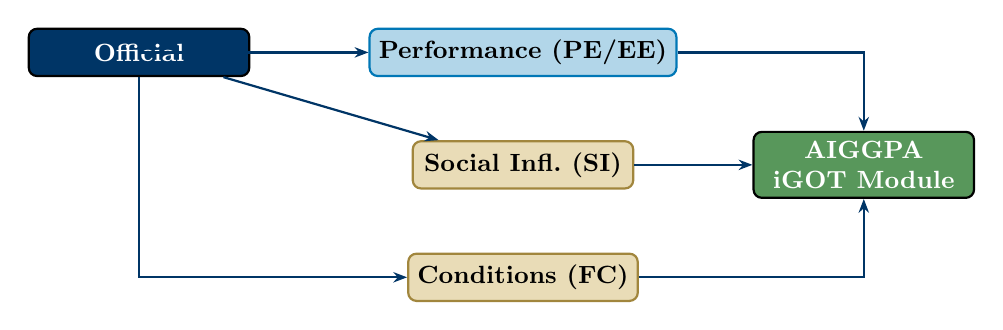
\begin{tikzpicture}[
  node distance=0.8cm and 1.5cm,
  box/.style={rectangle,rounded corners=3pt,minimum width=2.8cm,
    minimum height=0.6cm,align=center,font=\small\bfseries,
    draw,thick},
  arrow/.style={-{Stealth[length=5pt]},thick,color=navyblue}
]
  \node[box,fill=accentteal!30,draw=accentteal] (pe) {Performance (PE/EE)};
  \node[box,fill=navyblue,text=white,left=of pe] (input) {Official};
  \node[box,fill=gold!40,draw=gold!80!black,below=of pe] (si) {Social Infl.\ (SI)};
  \node[box,fill=gold!40,draw=gold!80!black,below=of si] (fc) {Conditions (FC)};
  \node[box,fill=darkgreen!80,text=white,right=of si] (out) {AIGGPA\\iGOT Module};

  \draw[arrow] (input) |- (pe);
  \draw[arrow] (input) -- (si);
  \draw[arrow] (input) |- (fc);
  \draw[arrow] (pe) -| (out);
  \draw[arrow] (si) -- (out);
  \draw[arrow] (fc) -| (out);
\end{tikzpicture}
\end{document}
